\documentclass[../../main.tex]{subfiles}
\begin{document}
In diesem Kapitel sei stets $K$ ein kommutativer Ring.

\section{Definition und Eigenschaften von Determinanten}

\begin{df}\label{9.1.1}
Sei $\si\in S_n$ [$\to$\ref{2.1.8}]. Ein \emph{Fehlstand}\index{Abbildung@{\bf Abbildung}!Permutation!Fehlstand} von $\si$ ist ein Paar $(i,j)\in\{1,\dots,n\}^2$ mit $i<j$ und $\si(i)>\si(j)$. Hat $\si$ genau $m$
Fehlstände, so definieren wir das \emph{Vorzeichen} (oder \emph{Signum}) von $\si$ durch $\sgn\si:=(-1)^m\in\{-1,1\}\subseteq\Z$.
\end{df}

\begin{bsp}\label{9.1.2}
$\si\colon\{1,\dots,5\}\to\{1,\dots,5\},\ 1\mapsto2,~2\mapsto3,~3\mapsto1,~4\mapsto5,~5\mapsto4$ hat genau die Fehlstände
$(1,3)$, $(2,3)$ und $(4,5)$ und daher Vorzeichen $(-1)^3=-1$.
\end{bsp}

\begin{df}\label{9.1.3}
Die Permutationen 
$$\ta_{k\ell}\colon\{1,\dots,n\}\to\{1,\dots,n\},\ i\mapsto\begin{cases}\ell&\text{falls }i=k\\k&\text{falls }i=\ell\\i&\text{sonst}\end{cases}$$
mit $k,\ell\in\{1,\dots,n\}$ und $k\ne\ell$ heißen \emph{Transpositionen}\index{Abbildung@{\bf Abbildung}!Permutation!Transposition}.
\end{df}

\begin{sat}\label{9.1.4}
$\forall\si,\ta\in S_n:\sgn(\si\circ\ta)=(\sgn\si)(\sgn\ta)$
\end{sat}

\begin{proof}
Ist $\rh\in S_n$, so gilt \[\sgn\rh=\prod_{i<j}\frac{\rh(j)-\rh(i)}{j-i},\]
denn das Produkt auf der rechten Seite hat wegen $\prod_{i<j}|\rh(j)-\rh(i)|=\prod_{i<j}|j-i|$ den Betrag $1$ und hat gleichzeitig
dasselbe Vorzeichen wie $\sgn\rh$, da der Faktor $\frac{\rh(j)-\rh(i)}{j-i}$ genau dann negativ ist, wenn $(i,j)$ ein Fehlstand ist.
Nun gilt
\begin{align*}
\sgn(\si\circ\ta)&=\prod_{i<j}\frac{\si(\ta(j))-\si(\ta(i))}{j-i}\\
&=\prod_{i<j}\frac{\si(\ta(j))-\si(\ta(i))}{\ta(j)-\ta(i)}\prod_{i<j}\frac{\ta(j)-\ta(i)}{j-i}=(\sgn\si)(\sgn\ta),
\end{align*}
wobei das Produkt $\prod_{i<j}\frac{\si(\ta(j))-\si(\ta(i))}{\ta(j)-\ta(i)}$ deswegen gleich $\sgn\si$ ist, weil in der Liste
\[(\ta(1),\ta(2)),(\ta(1),\ta(3)),(\ta(1),\ta(4)),\dots,(\ta(1),\ta(n)),\quad\dots\quad,(\ta(n-1),\ta(n))\]
für jedes $(i,j)\in\{1,\dots,n\}$ entweder genau einmal $(i,j)$ oder genau einmal $(j,i)$ auftaucht (ob ersteres oder letzteres ist egal wegen
$\frac{\si(j)-\si(i)}{j-i}=\frac{\si(i)-\si(j)}{i-j}$).
\end{proof}

\begin{kor}\label{9.1.5}
Jede Transposition hat Vorzeichen $-1$.
\end{kor}

\begin{proof}
Sei $\ta_{k\ell}\in S_n$ eine Transposition. Dann kann man $\si\in S_n$ wählen mit $\si(k)=1$ und $\si(\ell)=2$. Es gilt dann $\si\circ\ta_{k\ell}=\ta_{12}\circ\si$.
Mit \ref{9.1.4} erhält man daraus $(\sgn\si)(\sgn\ta_{k\ell})=(\sgn\ta_{12})(\sgn\si)$ und somit $\sgn\ta_{k\ell}=\sgn\ta_{12}$. Nun hat aber $\ta_{12}$ nur
den Fehlstand $(1,2)$ und daher Vorzeichen $-1$.
\end{proof}

\red{Bis hierher sollten wir am 17. Januar kommen.}

\begin{lem}\label{9.1.6}
Jede Permutation $\si\in S_n$ ist Hintereinanderschaltung \emph{[$\to$\ref{2.1.7}]} endlich vieler Transpositionen.
\end{lem}

\begin{proof}
Dies entspricht der Tatsache, dass man $n$ nebeneinander angeordnete Objekte durch paarweise Vertauschungen in jede beliebige Reihenfolge bringen kann.
\end{proof}

\begin{sat}\label{9.1.7}
Für jedes $n\in\N_0$ und $e\in K$ gibt es genau eine Funktion $\de_e^{(n)}\colon K^{n\times n}\to K$ mit folgenden Eigenschaften:
\begin{enumerate}[\rm(a)]
\item Für alle $i\in\{1,\dots,n\}$ und Zeilen
$a_1,\dots,a_{i-1},b,c,a_{i+1},\dots,a_n\in K^n$ gilt
\[\de_e^{(n)}\begin{pmatrix}a_1\\\vdots\\a_{i-1}\\b+c\\a_{i+1}\\\vdots\\a_n\end{pmatrix}=
\de_e^{(n)}\begin{pmatrix}a_1\\\vdots\\a_{i-1}\\b\\a_{i+1}\\\vdots\\a_n\end{pmatrix}+
\de_e^{(n)}\begin{pmatrix}a_1\\\vdots\\a_{i-1}\\c\\a_{i+1}\\\vdots\\a_n\end{pmatrix}\]
\item Für alle $i\in\{1,\dots,n\}$,
$a_1,\dots,a_n\in K^n$ und $\la\in K$ gilt
\[\de_e^{(n)}\begin{pmatrix}a_1\\\vdots\\a_{i-1}\\\la a_i\\a_{i+1}\\\vdots\\a_n\end{pmatrix}=
\la\de_e^{(n)}\begin{pmatrix}a_1\\\vdots\\a_{i-1}\\a_i\\a_{i+1}\\\vdots\\a_n\end{pmatrix}.\]
\item Für alle $A\in K^{n\times n}$ mit zwei identischen Zeilen gilt $\de_e^{(n)}(A)=0$.
\item $\de_e^{(n)}(I_n)=e$
\end{enumerate}
Es gilt
\begin{equation}\label{leibniz}\tag{$*$}\de_e^{(n)}(A)=e\sum_{\si\in S_n}(\sgn\si)a_{1\si(1)}\dotsm a_{n\si(n)}
\end{equation}
für alle $A=(a_{ij})_{1\le i,j\le n}\in K^{n\times n}$.
\end{sat}

\begin{proof}
Schreibe $e_j:=(0,\dots,0,\overbrace1^{\text{$j$-te Stelle}},0\dots,0)\in K^n$ für $j\in\{1,\dots,n\}$. Wir zeigen:
\begin{enumerate}[(1)]
\item Für jedes $\de_e^{(n)}\colon K^{n\times n}\to K$ mit (a)--(d) gilt \eqref{leibniz}.
\item $\de_e^{(n)}\colon K^{n\times n}\to K$ definiert durch \eqref{leibniz} erfüllt (a)--(d).
\end{enumerate}
\textbf{Zu (1).} Es habe $\de:=\de_e^{(n)}\colon K^{n\times n}\to K$ die Eigenschaften (a)--(d). Geht $B$ aus $A$ durch Vertauschen zweier Zeilen hervor,
so gilt $\de(B)=-\de(A)$, denn sind $a,b\in K^n$ diese zwei Zeilen, so gilt
\[0\overset{(c)}=\de\begin{pmatrix}\vdots\\a+b\\\vdots\\a+b\\\vdots\end{pmatrix}\overset{(a)}=
\de\underbrace{\begin{pmatrix}\vdots\\a\\\vdots\\a\\\vdots\end{pmatrix}}_{=0 \text{ nach (c)}}+
\de\begin{pmatrix}\vdots\\a\\\vdots\\b\\\vdots\end{pmatrix}+
\de\begin{pmatrix}\vdots\\b\\\vdots\\a\\\vdots\end{pmatrix}+
\de\underbrace{\begin{pmatrix}\vdots\\b\\\vdots\\b\\\vdots\end{pmatrix}}_{=0 \text{ nach (c)}}.\]
Mit \ref{9.1.6}, \ref{9.1.5} und \ref{9.1.4} folgt daraus für alle $\si\in S_n$
\[\de\begin{pmatrix}e_{\si(1)}\\\vdots\\e_{\si(n)}\end{pmatrix}=(\sgn\si)~\de\begin{pmatrix}e_1\\\vdots\\e_n\end{pmatrix}.\]
Sei nun $A=(a_{ij})_{1\le i,j\le n}\in K^{n\times n}$. Dann
\begin{eqnarray*}
\de(A)&=&\de\begin{pmatrix}\sum_{j=1}^na_{1j}e_j\\\vdots\\\sum_{j=1}^na_{nj}e_j\end{pmatrix}\overset{(a)}{\underset{(b)}=}
\sum_{j_1=1}^n\ldots\sum_{j_n=1}^na_{1j_1}\dotsm a_{nj_n}\de\begin{pmatrix}e_{j_1}\\\vdots\\e_{j_n}\end{pmatrix}\\
&\overset{(c)}=&\sum_{\si\in S_n}a_{1\si(1)}\dotsm a_{n\si(n)}\de\begin{pmatrix}e_{\si(1)}\\\vdots\\e_{\si(n)}\end{pmatrix}=
e\sum_{\si\in S_n}(\sgn\si)a_{1\si(1)}\dotsm a_{n\si(n)}.
\end{eqnarray*}
\textbf{Zu (2).} Für $\de:=\de_e^{(n)}$ definiert durch \eqref{leibniz} sind (a),(b) und (d) unmittelbar einsichtig. Um (c) zu zeigen, sei $A\in K^{n\times n}$
derart, dass die $k$-te Zeile und $\ell$-te Zeile ($k\ne\ell$) von $A$ übereinstimmen. Definiere $A_n:=\{\si\in S_n\mid\sgn\si=1\}$ und beachte, dass
[$\to$\ref{9.1.4},~\ref{9.1.5}]
\[\Ph\colon A_n\to S_n\setminus A_n,\ \si\mapsto\si\circ\ta_{k\ell}\] eine Bijektion ist. Dann
\begin{align*}
\de(A)&\overset{(*)}=e\sum_{\si\in A_n}(a_{1\si(1)}\dotsm a_{n\si(n)}-a_{1(\si\circ\ta_{k\ell})(1)}\dotsm a_{n(\si\circ\ta_{k\ell})(n)})\\
&=e\sum_{\si\in A_n}\left(\prod_{i\in\{1,\dots,n\}\setminus\{k,\ell\}}a_{i\si(i)}\right)
\underbrace{(a_{k\si(k)}a_{\ell\si(\ell)}-\underbrace{a_{k\si(\ell)}}_{=a_{\ell\si(\ell)}}
\underbrace{a_{\ell\si(k)}}_{=a_{k\si(k)}})}_{=0}=0.
\end{align*}
\end{proof}

\begin{bem}\label{9.1.8}
\begin{enumerate}[\normalfont(a)]
\item In \ref{9.1.7} besagen (a) und (b), dass $\de_e^{(n)}$ \emph{linear in den Zeilen} ist, das heißt der Wert einer Matrix unter $\de_e^{(n)}$ hängt linear von einer
Zeile ab, wenn man alle anderen Zeilen fixiert.
\item \ref{9.1.7}\eqref{leibniz} nennt man auch die \emph{Leibniz-Regel} [\href{http://de.wikipedia.org/wiki/Gottfried_Wilhelm_Leibniz}{Gottfried Wilhelm von Leibniz} *1646 \dag1716].
\end{enumerate}
\end{bem}

\begin{df}\label{9.1.9}
Sei $n\in\N_0$ und $A=(a_{ij})_{1\le i,j\le n}\in K^{n\times n}$. Dann heißt \[\det(A):=\de_1^{(n)}(A)\overset{\ref{9.1.7}\eqref{leibniz}}=\sum_{\si\in S_n}(\sgn\si)
a_{1\si(1)}\dotsm a_{n\si(n)}\] die \emph{Determinante}\index{Matrix@{\bf Matrix}!Determinante} von $A$.
\end{df}

\begin{bsp}\label{9.1.10}
\begin{enumerate}[\normalfont(a)]
\item $\det()=\de_1^{(0)}()\overset{()=I_0}=\de_1^{(0)}(I_0)\overset{\ref{9.1.7}(d)}=1$
\item Die Determinante einer Matrix, die eine Nullzeile enthält, ist null. Dies folgt zum Beispiel aus \ref{9.1.7}(b). Insbesondere gilt für die Nullmatrix
$0\in K^{n\times n}$ im Fall $n\ge1$, dass $\det(0)=0$ (nicht allerdings, wenn $n=0$ und $0\ne1$ in $K$, wie in (a) gesehen).
\item $\det(a)=a$ für alle $a\in K$
\item Sind $a,b,c,d\in K$, so $\det\begin{pmatrix}a&b\\c&d\end{pmatrix}=ad-bc$.
\item Sind $a,b,c,d,e,f,g,h,i\in K$, so gilt
\[\det\begin{pmatrix}a&b&c\\d&e&f\\g&h&i\end{pmatrix}=aei-afh-bdi+bfg+cdh-ceg.\]
\begin{center}
\begin{tikzcd}
\arrow[-,blue]{rd}&\arrow[-,blue]{rd}&\arrow[-,blue]{rd}&&\textcolor{red}-&\textcolor{red}-&\textcolor{red}-\\
&a\arrow[-,blue]{rd}&b\arrow[-,blue]{rd}&c\arrow[red]{ru}\arrow[-,blue]{rd}&\textcolor{Olive}a\arrow[red]{ru}&\textcolor{Olive}b\arrow[red]{ru}&\\
&d&e\arrow[-,red]{ru}\arrow[-,blue]{rd}&f\arrow[-,red]{ru}\arrow[-,blue]{rd}&\textcolor{Olive}d\arrow[-,red]{ru}\arrow[-,blue]{rd}&\textcolor{Olive}e&\\
&g\arrow[-,red]{ru}&h\arrow[-,red]{ru}&i\arrow[-,red]{ru}\arrow[blue]{rd}&\textcolor{Olive}g\arrow[blue]{rd}&\textcolor{Olive}h\arrow[blue]{rd}&\\
\arrow[-,red]{ru}&\arrow[-,red]{ru}&\arrow[-,red]{ru}&&\textcolor{blue}+&\textcolor{blue}+&\textcolor{blue}+&
\end{tikzcd}
Regel von Sarrus
\end{center}
\end{enumerate}
\end{bsp}

\begin{sat}\label{9.1.11}
Sei $A\in K^{n\times n}$ von der Gestalt
\begin{center}
$A=
\begin{pmatrix}~
\begin{tikzpicture}[inner sep=0]
\node[draw,regular polygon,regular polygon sides=4,inner sep=0,scale=1.2] (a1) {$A_1$};
\node[draw,regular polygon,regular polygon sides=4,inner sep=0] (a2) at (a1.south east) [anchor=north west] {$A_2$};
\node[draw,regular polygon,regular polygon sides=4,inner sep=0,scale=1.3] (am) at (1.5,-1.5) [anchor=north west] {$A_m$};
\node[scale=7] at (a2.north-|am) {$*$};
\node[scale=4.5] at (0.1,-1.9) {$0$};
\draw[loosely dotted,very thick,dash phase=2pt] (a2)--(am);
\end{tikzpicture}
\end{pmatrix}
$
mit quadratischen Matrizen $A_i$.
\end{center}
Dann gilt $\det A=\prod_{i=1}^m\det A_i$. Insbesondere ist die Determinante einer Matrix $A$ in
\emph{oberer Dreiecksgestalt}
$A=\begin{pmatrix}~
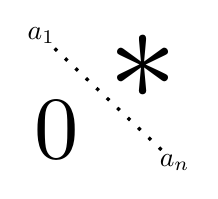
\begin{tikzpicture}[inner sep=0]
\node (a1) {$a_1$};
\node (an) at (1.5,-1.5) [anchor=north west] {$a_n$};
\node[scale=5] at (1.3,-0.4) {$*$};
\node[scale=3.2] at (0.2,-1.2) {$0$};
\draw[loosely dotted,very thick,dash phase=3pt] (a1)--(an);
\end{tikzpicture}
\end{pmatrix}
$ das Produkt ihrer \emph{Diagonaleinträge}, das heißt $\det A=\prod_{i=1}^na_i$.
\end{sat}

\begin{proof}
Es reicht, für $A=
\left(
\begin{array}{c|c}
B&*\\
\hline
0&C
\end{array}
\right)
$ mit $B\in K^{r\times r}$ und $C\in K^{t\times t}$ zu zeigen
\[\det A=(\det B)(\det C),\] denn der Rest folgt dann mit Induktion. Wegen der Nulleinträge links unten sind in der Leibniz-Formel \ref{9.1.7}\eqref{leibniz} nur diejenigen Summanden ungleich null, die zu einem $\si\in S_n$ gehören, für welches es $\rh\in S_r$ und $\ta\in S_t$ gibt mit $\si(i)=\rh(i)$ für $i\in\{1,\dots,r\}$ und
$\si(i)=\ta(i-r)+r$ für $i\in\{r+1,\dots,n\}$ (beachte $r+t=n$). Dabei ist die Anzahl der Fehlstände [$\to$\ref{9.1.1}] von $\si$ offensichtlich die Summe der Anzahl der
Fehlstände von $\rh$ und $\ta$, weswegen $\sgn\si=(\sgn\rh)(\sgn\ta)$ gilt. Es folgt
\[\det A=\sum_{\rh\in S_r}\sum_{\ta\in S_t}(\sgn\rh)(\sgn\ta)b_{1\rh(1)}\dotsm b_{r\rh(r)}c_{1\ta(1)}\dotsm c_{t\ta(t)},\]
wobei $B=(b_{ij})_{1\le i,j\le r}$ und $C=(c_{ij})_{1\le i,j\le t}$. Daher gilt
\[\det A=\left(\sum_{\rh\in S_r}(\sgn\rh)b_{1\rh(1)}\dotsm b_{r\rh(r)}\right)\left(\sum_{\ta\in S_t}(\sgn\ta)c_{1\ta(1)}\dotsm c_{t\ta(t)}\right)
\overset{\ref{9.1.7}\eqref{leibniz}}=(\det B)(\det C).\]
\end{proof}

\begin{bem}\label{9.1.12}
Sei $K$ ein Körper. Zur Berechnung von Determinanten ist es oft am effizientesten, die Matrix durch Zeilenoperationen [$\to$§\ref{5.2}] auf obere Dreiecksgestalt (zum Beispiel Stufenform [$\to$\ref{5.1.10}]) zu bringen und den Effekt auf die Determinante dabei mitzuprotokollieren. Für die beiden \emph{elementaren} Zeilenoperationen [$\to$\ref{5.2.1}] gilt:
\begin{enumerate}[\normalfont(a)]
\item Sind $A,B\in K^{n\times n}$ mit $A\overset{Z_i\leftarrow Z_i+\la Z_j}\sim B$ ($i,j\in\{1,\dots,n\},i\ne j,\la\in K$), so gilt $\det A=\det B$ [$\to$\ref{9.1.7}(a)--(c)].
\item Sind $A,B\in K^{n\times n}$ mit $A\overset{Z_i\leftarrow\la Z_i}\sim B$ ($i\in\{1,\dots,n\},\la\in K^\times$), so gilt $\det A=\frac1\la\det B$ [$\to$\ref{9.1.7}(b)].
\end{enumerate}
Daraus ergibt sich der Effekt auf andere Zeilenoperationen:
\begin{enumerate}[\normalfont(a)]
\item[(c)] Sind $A,B\in K^{n\times n}$ mit $A\overset{Z_i\leftrightarrow Z_j}\sim B$ ($i,j\in\{1,\dots,n\},i\ne j$), so gilt $\det A=-\det B$ [durch Simulation wie in \ref{5.2.1} aus (a) und (b)
oben oder wie im Beweis von \ref{9.1.7}].
\item[(d)] Sind $A,B\in K^{n\times n}$ mit $A\overset{Z_i\leftarrow\sum_{j=1}^n\la_jZ_j}\sim B$ ($i\in\{1,\dots,n\},\la_1,\dots,\la_n\in K,\la_i\ne0$), so gilt $\det A=\frac1{\la_i}\det B$ [durch Simulation wie in \ref{5.2.1} aus (a) und (b) oben].
\end{enumerate}
\end{bem}

\begin{bsp}\label{9.1.13}
Sei $K$ ein Körper, schreibe $2:=1+1\in K$ und so weiter. Gelte $3\in K^\times$.
\begin{multline*}
A:=\begin{pmatrix}1&2&-1&0\\2&3&0&1\\-1&1&1&0\\0&9&3&-3\end{pmatrix}
\overset{Z_2\leftarrow Z_2-2Z_1}{\underset{Z_3\leftarrow Z_3+Z_1}\sim}
\begin{pmatrix}1&2&-1&0\\0&-1&2&1\\0&3&0&0\\0&9&3&-3\end{pmatrix}\\
\overset{\over{
\tikz[baseline]{
            \node[fill=blue!10,draw,ellipse,anchor=base,inner sep=0] (t1)
            {$\scriptstyle Z_4\leftarrow\frac13Z_4$};
        }
}{\scriptstyle Z_4\leftarrow Z_4-Z_3}}{\underset{Z_3\leftarrow Z_3+3Z_2}\sim}
\begin{pmatrix}1&2&-1&0\\0&-1&2&1\\0&0&6&3\\0&0&1&-1\end{pmatrix}
\overset{
\tikz[baseline]{
            \node[fill=red!10,draw,anchor=base] (t3)
            {$\scriptstyle Z_3\leftrightarrow Z_4$};
        }
}
{\underset{Z_4\leftarrow Z_4-6Z_3}\sim}
\begin{pmatrix}
\tikz[baseline=(t5.base)]\node (t5){$1$};
&2&-1&0\\0&-1&2&1\\0&0&1&-1\\0&0&0&\tikz[baseline=(t6.base)]\node (t6){$9$};\end{pmatrix}=:B
\end{multline*}
Also $\det A\overset{\ref{9.1.7}(b)(c)}=
\tikz[baseline]{
            \node[fill=blue!10,draw,ellipse,anchor=base,inner sep=0] (t2)
            {$\frac1{\frac13}$};
        }
\tikz[baseline]{
            \node[fill=red!10,draw,anchor=base,inner sep=0.2] (t4)
            {$(-1)$};
        }
\det B=(-3)
\tikz[baseline]{
            \node[fill=orange!10,draw,ellipse,circle,anchor=base,inner sep=0] (t8)
            {$(-9)$};
        }
=27$.
\begin{tikzpicture}[overlay]
        \path[->] (t1.west) edge [line width=0.7mm,color=blue,bend right=40] (t2.north west);
        \path[->] (t3.south west) edge[line width=0.7mm,color=red,bend left=20] (t4.north east);
        \draw[opacity=.5,line width=5 mm,line cap=round,color=orange] (t5.center) to node(t7){} (t6.center);
                \path[->] (t7) edge[line width=0.7mm,color=orange,bend left=55] (t8);
\end{tikzpicture}
\end{bsp}

\begin{bem}\label{9.1.14}
Sei $K$ ein Körper und $A\in K^{n\times n}$. Ist $A$ in Stufenform [$\to$\ref{5.1.10}], so ist der Rang von $A$ [$\to$\ref{8.1.14}] gleich der Anzahl der Stufen von $A$ und die Determinante
von $A$ [$\to$\ref{9.1.9}] gleich dem Produkt der Diagonaleinträge von $A$ [$\to$\ref{9.1.11}].
Es gilt dann
\[\rank A=n\iff\det A\ne0.\]
Dies bleibt richtig für beliebiges $A\in K^{n\times n}$, denn durch Zeilenoperationen ändert sich der Rang gar nicht [$\to$\ref{6.2.29}(c)] und die Determinante nur um einen Faktor
$\ne0$ [$\to$\ref{9.1.12}]. Wegen $A$ invertierbar $\overset{\ref{8.1.16}}\iff\rank A=n$ und $K^\times=K\setminus\{0\}$ gilt also auch
\[A\text{ invertierbar}\iff\det A\in K^\times,\]
was wir in §9.2 sogar beweisen werden, wenn $K$ nur ein kommutativer Ring statt ein Körper ist.
\end{bem}

\begin{sat}[Determinantenproduktsatz]\label{9.1.15}
Für alle $A,B\in K^{n\times n}$ gilt \[\det(AB)=(\det A)(\det B).\]
\end{sat}

\begin{proof}
Sei $B\in K^{n\times n}$ fest und betrachte
\begin{align*}
f\colon K^{n\times n}\to K,&\ A\mapsto\det(AB)\qquad\text{ sowie}\\
g\colon K^{n\times n}\to K,&\ A\mapsto(\det A)(\det B).
\end{align*}
Zu zeigen ist $f=g$. Wir zeigen $f=\de_{\det B}^{(n)}=g$, indem wir die Eigenschaften \ref{9.1.7}(a)--(d) von $\de_{\det B}^{(n)}$ für $f$ und $g$ nachweisen. Für $g$ sind diese
Eigenschaften klar. Für $f$ rechnet man sie sofort nach, zum Beispiel (a):
\begin{multline*}
f\begin{pmatrix}a_1\\\vdots\\a_{i-1}\\b+c\\a_{i+1}\\\vdots\\a_n\end{pmatrix}=\det\begin{pmatrix}\begin{pmatrix}a_1\\\vdots\\a_{i-1}\\b+c\\a_{i+1}\\\vdots\\a_n\end{pmatrix}B\end{pmatrix}=\det\begin{pmatrix}a_1B\\\vdots\\a_{i-1}B\\(b+c)B\\a_{i+1}B\\\vdots\\a_nB\end{pmatrix}
=\det\begin{pmatrix}a_1B\\\vdots\\a_{i-1}B\\bB+cB\\a_{i+1}B\\\vdots\\a_nB\end{pmatrix}
\\\overset{\ref{9.1.7}(a)}=
\det\begin{pmatrix}a_1B\\\vdots\\a_{i-1}B\\bB\\a_{i+1}B\\\vdots\\a_nB\end{pmatrix}+
\det\begin{pmatrix}a_1B\\\vdots\\a_{i-1}B\\cB\\a_{i+1}B\\\vdots\\a_nB\end{pmatrix}=
f\begin{pmatrix}a_1\\\vdots\\a_{i-1}\\b\\a_{i+1}\\\vdots\\a_n\end{pmatrix}+
f\begin{pmatrix}a_1\\\vdots\\a_{i-1}\\c\\a_{i+1}\\\vdots\\a_n\end{pmatrix}
\end{multline*}
für alle $a_i,b,c\in K^n$.
\end{proof}

\red{Bis hierher sollten wir am 20. Januar kommen.}

\begin{df}\label{9.1.16}
Zwei Matrizen $A,B\in K^{n\times n}$ heißen \emph{ähnlich}\index{Matrix@{\bf Matrix}!Ähnlichkeit}, in Zeichen $A\approx B$, wenn es eine
invertierbare Matrix $P\in K^{n\times n}$ gibt mit $A=P^{-1}BP$.
\end{df}

\begin{pro}\label{9.1.17}
Ähnlichkeit ist eine Äquivalenzrelation auf $K^{n\times n}$.
\end{pro}

\begin{proof} Gemäß \ref{1.3.1}(b) ist zu zeigen:
\begin{enumerate}[\normalfont(a)]
\item $\forall A\in K^{n\times n}:A\approx A$
\item $\forall A,B\in K^{n\times n}:(A\approx B\implies B\approx A)$
\item $\forall A,B,C\in K^{n\times n}:((A\approx B\et B\approx C)\implies A\approx C)$
\end{enumerate}
\textbf{Zu (a).} $A=I_n^{-1}AI_n$ für alle $A\in K^{n\times n}$ [$\to$\ref{7.2.9}]

\medskip\noindent
\textbf{Zu (b).} Ist $P\in K^{n\times n}$ invertierbar mit $A=P^{-1}BP$, so ist auch $P^{-1}$ invertierbar und $B=PAP^{-1}=(P^{-1})^{-1}AP^{-1}$.

\medskip\noindent
\textbf{Zu (c).} Sind $P,Q\in K^{n\times n}$ invertierbar mit $A=P^{-1}BP$ und $B=Q^{-1}CQ$, so ist auch $QP$ invertierbar mit $(QP)^{-1}=P^{-1}Q^{-1}$
(denn $P^{-1}Q^{-1}QP=I_n=QPP^{-1}Q^{-1}$) und es gilt $A=P^{-1}Q^{-1}BQP=(QP)^{-1}B(QP)$.
\end{proof}

\begin{sat}\label{9.1.18}
Sind $A,B\in K^{n\times n}$ mit $A\approx B$, so gilt $\det A=\det B$.
\end{sat}

\begin{proof}
Seien $A,B\in K^{n\times n}$ mit $A\approx B$. Wähle $P\in K^{n\times n}$ invertierbar mit $A=P^{-1}BP$. Dann
$\det A\overset{\ref{9.1.15}}=(\det(P^{-1}))(\det B)(\det P)$ und
$$1\overset{\ref{9.1.9}}=\det I_n\overset{\ref{7.2.9}}=\det(P^{-1}P)\overset{\ref{9.1.15}}=(\det(P^{-1}))(\det P).$$
\end{proof}

\begin{pro}\label{9.1.19}
Sei $f$ ein Endomorphismus {\rm[$\to$\ref{6.3.1}]} eines endlichdimensionalen Vektorraums mit geordneten Basen $\v$ und $\w$. Dann $M(f,\v)\approx M(f,\w)$ {\rm[$\to$\ref{7.1.11}]}.
\end{pro}

\begin{proof}
Es gilt $M(f,\v)\overset{\ref{7.2.5}}=M(\w,\v)M(f,\w)M(\v,\w)$ und
\[I_n\underset{\ref{7.2.10}}{\overset{\ref{7.1.10}}=}M(\v,\v)\overset{\ref{7.2.5}}=M(\w,\v)M(\v,\w),\]
das heißt $M(\w,\v)=M(\v,\w)^{-1}$ [$\to$\ref{7.2.13}]. Mit $P:=M(\v,\w)$ gilt also \[M(f,\v)\overset{\ref{7.2.5}}=P^{-1}M(f,\w)P.\]
\end{proof}

\begin{df}\label{9.1.20}
Sei $f$ ein Endomorphismus eines endlichdimensionalen Vektorraums $V$. Dann ist die \emph{Determinante} von $f$ definiert als
$\det f:=\det M(f,\v)$, wobei $\v$ eine beliebig gewählte geordnete Basis von $V$ ist [$\to$\ref{6.2.22},~\ref{9.1.18}]
\end{df}

\begin{df}\label{9.1.21}
Ist $A=(a_{ij})_{1\le i\le m,1\le j\le n}\in K^{m\times n}$, so heißt \[A^T:=(a_{ij})_{1\le j\le n,1\le i\le m}\in K^{n\times m}\] die zu $A$ \emph{transponierte} Matrix.
\end{df}

\begin{bsp}\label{9.1.22}
$\begin{pmatrix}1&2\\0&1\\3&1\end{pmatrix}^T=\begin{pmatrix}1&0&3\\2&1&1\end{pmatrix}$
\end{bsp}

\begin{pro}\label{9.1.23}
$\forall A\in K^{n\times n}:\det A=\det(A^T)$
\end{pro}

\begin{proof}
Wegen $\si=(\si^{-1})^{-1}$ für alle $\si\in S_n$ ist $\Ph\colon S_n\to S_n,\si\mapsto\si^{-1}$ bijektiv. Es gilt
\begin{eqnarray*}
\det(A^T)&\overset{\ref{9.1.7}\eqref{leibniz}}=&\sum_{\si\in S_n}(\sgn\si)a_{\si(1)1}\dotsm a_{\si(n)n}\\
&\overset{\text{$\Ph$ bijektiv}}=&\sum_{\si\in S_n}(\sgn(\si^{-1}))a_{\si^{-1}(1)1}\dotsm a_{\si^{-1}(n)n}\\
&\underset{\text{für $\si\in S_n$}}{\overset{\text{$\si$ bijektiv}}=}&\sum_{\si\in S_n}(\sgn(\si^{-1}))a_{\si^{-1}(\si(1))\si(1)}\dotsm a_{\si^{-1}(\si(n))\si(n)}\\
&\underset{\text{da $(\sgn(\si^{-1}))(\sgn\si)=\sgn(\id)=1$}}{\overset{\sgn(\si^{-1})=\sgn\si}=}&
\sum_{\si\in S_n}(\sgn\si)a_{1\si(1)}\dotsm a_{n\si(n)}\overset{\ref{9.1.7}\eqref{leibniz}}=\det A
\end{eqnarray*}
\end{proof}

\begin{bem}\label{9.1.24}
Proposition \ref{9.1.23} hat offensichtliche Konsequenzen: Die Determinantenfunktion ist auch \emph{linear in den Spalten} [$\to$\ref{9.1.8}(a)], zur Berechnung
von Determinanten kann man auch (analog zu \ref{5.2.1} definierte) \emph{Spaltenoperationen} heranziehen [$\to$\ref{9.1.12}], die Determinante einer
Matrix in \emph{unterer} Dreiecksgestalt [$\to$\ref{9.1.11}] ist das Produkt ihrer Diagonaleinträge und so weiter.
\end{bem}

\section{Determinantenentwicklung und Komatrix}

\begin{sat}\label{9.2.1}
Sei $A = (a_{ij})_{1\le i,j\le n}\in K^{n\times n}$ und bezeichne $A_{ij}\in K^{(n-1)\times (n-1)}$ für $i,j\in \left\{1,\ldots,n\right\}$ die Matrix, die aus $A$ durch Streichen der $i$-ten Zeile und $j$-ten Spalte entsteht. \index{Matrix@{\bf Matrix}!Determinante!Entwicklung}
\begin{enumerate}[\rm(a)]
\item Für alle $i\in \left\{1,\ldots,n\right\}$ gilt
\[\det A = \sum_{j = 1}^{n}(-1)^{i+j}a_{ij} \det A_{ij}\]
"`Entwicklung nach der $i$-ten Zeile"'
\item Für alle $j\in \left\{1,\ldots,n\right\}$ gilt
\[\det A = \sum_{i = 1}^{n}(-1)^{i+j}a_{ij} \det A_{ij}\]
"`Entwicklung nach der $j$-ten Spalte"'
\end{enumerate}
\end{sat}
\begin{proof}
Wegen \ref{9.1.23} reicht es, (a) zu zeigen. Hierzu rechnet man
\begin{align*}
\det A & \overset{\text{\ref{9.1.7}(a)(b)}}= \sum_{j = 1}^{n} a_{ij} \det \left(
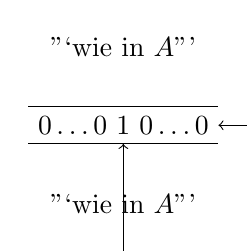
\begin{tikzpicture}[baseline={(current bounding box.center)}]
\node(O){"`wie in $A$"'};
\node[below of = O](M){$0\ldots0\ 1\ 0\ldots0$};
\node[below of = M]{"`wie in $A$"'};
\draw(M.south west)--(M.south east);
\draw(M.north west)--(M.north east);
\node[right of = M,xshift=1.2cm,overlay](I){$i$};
\node[below of = M,yshift=-1.2cm,overlay](J){$j$};
\draw[->,overlay](I.west)--(M.east);
\draw[->,overlay](J.north)--(M.south);
\end{tikzpicture}
\right)
\\[2cm]
&\overset{\text{\ref{9.1.12}(a)}}{=} \sum_{j = 1}^{n} a_{ij}
\det \left(
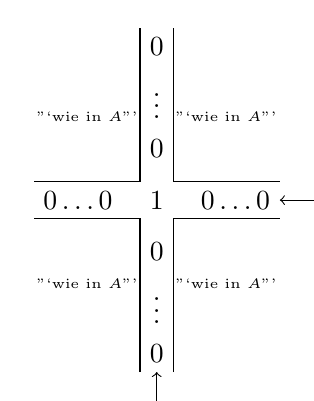
\begin{tikzpicture}[baseline={(current bounding box.center)}]
\node(ONE){$1$};
\node[left of = ONE](ONEL){$0 \ldots 0$};
\node[right of = ONE](ONER){$0 \ldots 0$};
\node[above of = ONE,yshift=-1em](OBEN1){$0$};
\node[below of = ONE,yshift=1em](UNTEN1){$0$};
\node[above of = OBEN1,yshift=-1em](OBEN2){$\vdots$};
\node[above of = OBEN2,yshift=-1em](OBEN3){$0$};
\node[below of = UNTEN1,yshift=1em](UNTEN2){$\vdots$};
\node[below of = UNTEN2,yshift=1em](UNTEN3){$0$};
\draw(OBEN3.north east)--(ONE.north east) -- (ONER.north east);
\draw(OBEN3.north west)--(ONE.north west) -- (ONEL.north west);
\draw(UNTEN3.south east)--(ONE.south east) -- (ONER.south east);
\draw(UNTEN3.south west)--(ONE.south west) -- (ONEL.south west);
\node[right of = ONER,xshift=1em,overlay](I){$i$};
\node[below of = UNTEN3,yshift=-1em,overlay](J){$j$};
\draw[->,overlay](I.west)--(ONER.east);
\draw[->,overlay](J.north)--(UNTEN3.south);
\node[above right of = ONE,xshift=0.5em,yshift=1em]{\tiny"`wie in $A$"'};
\node[above left of = ONE,xshift=-0.5em,yshift=1em]{\tiny"`wie in $A$"'};
\node[below left of = ONE,xshift=-0.5em,yshift=-1em]{\tiny"`wie in $A$"'};
\node[below right of = ONE,xshift=0.5em,yshift=-1em]{\tiny"`wie in $A$"'};
\end{tikzpicture}
\right)
\\[2cm]
& \overset{\text{\ref{9.1.12}(c)}}{=} \sum_{j = 1}^{n} a_{ij}\underbrace{(-1)^{(n-i)+(n-j)}}_{(-1)^{i+j}}\underbrace{\det \left(\begin{array}{c|c}
 & 0\\
A_{ij} & \vdots\\
& 0\\\hline
0\ldots 0 & 1
\end{array}\right)}_{\textstyle\overset{\text{\ref{9.1.11}}}{=}(\det A_{ij})\underbrace{\det (1)}_{=1}}
\end{align*}
\end{proof}

\begin{bsp}\label{9.2.2}
\begin{multline*}
\det\begin{pmatrix}
2 & 0 & 4 & \tikz[baseline=(m1.base)]\node[draw=blue, circle, inner sep = 2](m1){$1$};\\
1 & 9 & -1 & 0\\
0 & 1 & 1 & \tikz[baseline=(m2.base)]\node[draw=blue, ellipse, inner sep = 2](m2){$-3$};\\
-1 & 1 & 2 & 0
\end{pmatrix}\qquad\qquad\qquad\qquad\qquad\qquad\qquad\begin{pmatrix}
+ & - & + & \tikz[baseline=(p1.base)]\node[draw=red, circle, inner sep = 1](p1){$-$};\\
- & + & - & +\\
+ & - & + & \tikz[baseline=(p2.base)]\node[draw=red, circle, inner sep = 1](p2){$-$};\\
- & + & - & +
\end{pmatrix}\\
\overset{\text{Entwicklung nach}}{\underset{\text{letzter Spalte}}{=}} \tikz[baseline=(g1.base)]\node[fill=red!20, inner sep = 0, ellipse, draw](g1){$-$}; \tikz[baseline=(g2.base)]\node[fill=blue!20, inner sep = 0, ellipse, draw](g2){$1$};\underbrace{\det\begin{pmatrix}
1 & 9 & -1\\
0 & 1 & 1\\
-1 & 1 & 2
\end{pmatrix}}_{\llap{$\begin{array}{l}
\scriptstyle\overset{\text{Entwicklung nach}}{\underset{\text{erster Spalte}}{=}} \det \left(\begin{smallmatrix}
1 & 1 \\
1 & 2 
\end{smallmatrix}\right)- \det\left(\begin{smallmatrix}
9 & -1 \\
1 & 1
\end{smallmatrix}\right)\\
\scriptstyle\qquad\qquad= (2-1)-(9+1)= -9\end{array}$}}\tikz[baseline=(g3.base)]\node[fill=red!20, inner sep = 0, ellipse, draw](g3){$-$}; \tikz[baseline=(g4.base)]\node[fill=blue!20, inner sep = 0, ellipse, draw](g4){$(-3)$};\underbrace{\det \begin{pmatrix}
2 & 0 & 4\\
1 & 9 & -1\\
-1 & 1 & 2
\end{pmatrix}}_{\rlap{$\begin{array}{l}
\scriptstyle\overset{\text{Entwicklung nach}}{\underset{\text{erster Zeile}}{=}} 2\det\left(\begin{smallmatrix}
9 & -1\\
1 & 2
\end{smallmatrix}\right)+ 4\det \left(\begin{smallmatrix}
1 & 9\\
-1 & 1
\end{smallmatrix}\right)\\
\scriptstyle\qquad\qquad= 2\cdot 19 + 4\cdot 10= 78
\end{array}$}}= 9 + 3\cdot 78 = 243
\begin{tikzpicture}[overlay]
\path (p1) edge [->, very thick, red, bend right=20] (g1.north);
\path (p2) edge [->, very thick, red, bend right=20] (g3.north);
\path (m1) edge [->, very thick, blue, bend left=40] (g2);
\path (m2) edge [->, very thick, blue, bend left=20] (g4);
\end{tikzpicture}
\end{multline*}
\end{bsp}

\begin{df}\label{9.2.3}
Ist $A=(a_{ji})_{1\le i,j\le n}\in K^{n\times n}$ und bezeichnet $A_{ij}\in K^{(n-1)\times (n-1)}$ für $i,j\in \left\{1,\ldots,n\right\}$ wieder die Matrix, die aus $A$ durch Streichen der $i$-ten Zeile und $j$-ten Spalte entsteht, so nennt man \[\com A := \left((-1)^{i+j}\det A_{ij}\right)_{1\le i,j\le n}\] die \emph{Komatrix}\index{Matrix@{\bf Matrix}!Komatrix} von $A$.
\end{df}

\begin{sat}\label{9.2.4}
Sei $A\in K^{n\times n}$. Dann \[A(\com A)^T = (\det A)I_n = (\com A)^TA.\]
\end{sat}
\begin{proof}
Es gilt $(\com A)^T = \left((-1)^{i+j}\det A_{ji}\right)_{1\le i,j\le n}$ [$\to$ \ref{9.1.21}, \ref{9.2.3}]. Schreibe $I_n = \left(\delta_{ij}\right)_{1\le i,j\le n}$. Seien $i,k\in \left\{1\ldots,n\right\}$. Nach \ref{7.2.1} ist zu zeigen:
$$\sum_{j= 1}^{n} a_{ij}(-1)^{j+k}\det A_{kj} = (\det A)\delta_{ik} = \sum_{j = 1}^{n}(-1)^{i+j}(\det A_{ji})a_{jk}.$$
Für $i = k$ steht \case{links}{rechts} die Entwicklung der Determinante von $A$ nach der $k$-ten \case{Zeile}{Spalte}.
Für $i\ne k$ steht \case{links}{rechts} die Entwicklung der Determinante einer Matrix, deren $i$-te und $k$-te \case{Zeile}{Spalte} übereinstimmen nach der
\case{$k$-ten Zeile}{$i$-ten Spalte}.
\end{proof}

\begin{kor}[in \ref{9.1.14} schon bewiesen, falls $K$ ein Körper]\label{9.2.5}
Eine Matrix $A\in K^{n\times n}$ ist invertierbar genau dann, wenn $\det A \in K^{\times}$. In diesem Fall gilt $A^{-1} = (\det A)^{-1}(\com A)^T$.
\end{kor}
\begin{proof}
Ist $A$ invertierbar [$\to$ \ref{7.2.9}], so $1=\det I_n = \det(A A^{-1}) \overset{\ref{9.1.15}}{=} (\det A)(\det (A^{-1}))$, also $\det A\in K^\times$. Ist $\det A\in K^\times$, so $A\left(\frac{1}{\det A}(\com A)^T\right) \overset{\ref{9.2.4}}{=} I_n \overset{\ref{9.2.4}}{=}\left(\left(\frac{1}{\det A}\right)(\com A)^T\right) A$.
\end{proof}

\begin{kor}[in \ref{7.2.13} schon bewiesen, falls $K$ Körper]\label{9.2.6}
Seien $A,B\in K^{n\times n}$. Dann $AB = I_n\iff BA = I_n$.
\end{kor}
\begin{proof}
Gelte $AB = I_n$. Dann $(\det A)(\det B) = 1$ nach \ref{9.1.15}. Also $\det B\in K^\times$ und nach \ref{9.2.5} ist $B$ invertierbar. Dann aber
$$BA = BA(BB^{-1}) = B(AB)B^{-1} = BB^{-1} = I_n$$
wie im Beweis von \ref{7.2.13}.
\end{proof}

\begin{sat}[Cramersche Regel {[\href{http://de.wikipedia.org/wiki/Gabriel_Cramer}{Gabriel Cramer} *1704, \dag 1752]}]\label{9.2.7}
Seien $A\in K^{n\times n}$ und $x,b\in K^n$ mit $Ax = b$ {\rm[$\to$ §\ref{7.3}]}. Bezeichne $A_i\in K^{n\times n}$ für $i\in \left\{1,\ldots,n\right\}$ die Matrix, die aus $A$ entsteht, indem man die $i$-te Spalte durch $b$ ersetzt. Dann
$$(\det A)x_i = \det A_i \qquad\text{für }i\in \left\{1,\ldots,n\right\}.$$
\end{sat}
\begin{proof}
Für $X_i := \left(\begin{array}{cc|c|cc}
1 & & x_1 & \\
 & \ddots & \vdots & \multicolumn{2}{c}{\text{{\tiny"`wie in $I_n$"'}}}\\
 & & x_i & \\
 \multicolumn{2}{c|}{\text{{\tiny"`wie in $I_n$"'}}} & \vdots & \ddots\\
 & & x_n & & 1
\end{array}\right)$ gilt
$$\det X_i \overset{\ref{9.1.12}\text{(a)}}{\underset{\ref{9.1.24}}{=}} \det
\begin{pmatrix}
1\\
&\ddots\\
&&1\\
&&&\tikz\node(P192){$x_i$};\\
&&&&1\\
&&&&&\ddots\\
&&&&&&1
\end{pmatrix}
\begin{tikzpicture}[overlay]
\node[below left of = P192,xshift=-1em,yshift=-1em,scale=5]{$0$};
\node[above right of = P192,xshift=1em,yshift=1em,scale=5]{$0$};
\end{tikzpicture}
 \overset{\ref{9.1.11}}{=}x_i$$
sowie $AX_i \overset{Ax = b}{\underset{\ref{7.2.2}\text{(c)}}{=}} A_i$ und daher
\[(\det A)x_i = (\det A)(\det X_i) = \det(AX_i) = \det(A_i)\]
für $i\in\{1,\ldots,n\}$.
\end{proof}

\red{Bis hierher sollten wir am 24. Januar kommen.}

\end{document}